\section{Rozbor tématu a použitých metod/technologií}\label{chap:analysis}

\subsection{Sumarizace faktů}



\subsubsection{Návštěvníci chaty}

Slovinské hory navštíví ročně kolem 1.7 milionu turistů.\footnote{\url{https://www.rtvslo.si/news-in-english/every-year-1-7-million-hikers-visit-slovenia-s-mountains/462870}}. Drtivá většina takto učiní v hlavní sezóně, období červen -- září. V době Slovinských prázdnin je pak špička úplně největší a na Triglav vystoupá až 2000 lidí za víkend.\footnote{\url{https://www.explore-share.com/blog/climbing-mount-triglav-slovenia/}} Po zbytek hlavní sezóny uvažujeme 1500 lidí za víkend. Ve všední dny pak počítáme s polovinou turistů. Délka hlavní sezóny jsou 4 měsíce (17 týdnů).

$8.5*2*1000=17000$\\
$8.5*5*500=21250$\\
$8.5*2*750=12750$\\
$8.5*5*375=15937$\\
$17000+21250+12750+15937=66937$\\
$66937/(17*7)=562$

V průběhu hlavní sezóny navštíví Triglav kolem \textbf{562} lidí denně. Mimo sezónu uvažujeme desetinu turistů, tedy \textbf{56} lidí denně.

Kapacita chaty pro přenocování je až \textbf{350} lidí. Restaurace může pojmout naráz zhruba \textbf{50} zákazníků.\footnote{\url{https://www.summitpost.org/kredarica-hut-triglavski-dom-na-kredarici/349588}}

Na úpatí hory jsou další dvě chaty, ty jsou ale podstatně menší a mají menší kapacitu. Předpokládáme, že Triglavski Dom navštíví \textbf{2/3} všech turistů. Na Triglav vede mnoho cest. Všechny jsou standardně dvoudenní, pouze velmi zkušení horolezci zvládnou celý výstup za jeden den.\footnote{\url{https://www.hedvabnastezka.cz/zeme/evropa/slovinsko/29363-vystup-na-triglav-cestou-cez-prag-trail/}} Jelikož Triglav je hora pro širší veřejnost, uvažujeme, že pro přenocování se rozhodne \textbf{4/5} turistů. Ty na chatě zůstanou dobu definovanou normálním rozdělením se středem \textbf{12} hodin. Zbytek se na chatě zastaví pouze krátce, dobu definovanou normálním rozdělením se středem \textbf{3} hodiny.

Bereme v potaz i situaci, kdy by na chatě nešla elektřina. To by znamenalo značné omezení fungovaní restaurace a hlavně zimu. Předpokládáme, že by to malé množství návštěvníků chaty odradilo. Buď by se na základě toho rozhodli pro jednodenní výstup, využili by služeb jiné chaty, nebo se vrátili zpět do údolí. Takto by se podle našich odhadů zachovalo \textbf{10\%} zákazníků.



\subsubsection{Spotřeba energie}

Na základě grafu\footnote{\url{https://www.statista.com/statistics/195728/average-energy-consumption-per-guest-night-in-hotels-by-continent/}} jsme určili spotřebu energie hosta za noc. Bude se řídit normálním rozdělením se středem \textbf{20\,kWh} (70MJ). Bereme výrazně nižší hodnotu, než je průměr, protože se jedná o horskou chatu, ne standardní hotel. U návštěvníků, kteří se zastaví pouze na kratší odpočinek bude spotřeba velmi nízká a uvažujeme normální rozložení se středem \textbf{5\,kWh} (70MJ).

Chata sama o sobě spotřebuje nějakou energii, i bez zákazníků. Například topit a svítit se bude do jisté míry i pro personál. Průměrný americký hotel spotřebuje 14\,kWh na $ft^2$ ročně.\footnote{\url{https://www.mge.com/saving-energy/business/bea/article_detail.htm}} Na základě této úměry odhadujeme spotřebu naší chaty na \textbf{180\,kWh} denně.



\subsubsection{Větrné turbíny}

Větrné turbíny začínají produkovat energii při rychlosti větru 4 až 5 metrů za sekundu a maximálního výkonu dosahují při rychlosti 15 metrů za sekundu. Naopak při velmi silném větru nad 25 metrů za sekundu se turbíny vypínají.\footnote{\url{http://www.ewea.org/wind-energy-basics/faq/}} Na základě informací z\footnote{\url{https://www.engineering.com/ElectronicsDesign/ElectronicsDesignArticles/ArticleID/9556/Rooftop-Wind-Turbines-Are-They-Worthwhile.aspx}} \footnote{\url{https://www.meteoblue.com/en/weather/forecast/modelclimate/kredarica_slovenia_3197311}} jsme sestavili tabulku~\ref{tab:wind_energy} produkce energie turbíny dle síly větru.

\begin{center}
    \begin{table}[!h]
        \centering
        \begin{tabular}{|c|c|}
            \hline
            Síla větru [km/hod] & Produkce energie jedné turbíny [$kWh/$hod] \\
            \hline
            \hline
            0 - 4.5 & 0 \\
            \hline
            4.5 - 10 & 0.1 \\
            \hline
            10 - 20 & 0.2 \\
            \hline
            20 - 30 & 0.4 \\
            \hline
            30 - 54 & 0.8 \\
            \hline
            54 - 90 & 1 \\
            \hline
            90 + & 0 \\
            \hline
        \end{tabular}
        \caption{Produkce energie vetrné turbíny v závislosti na síle větru}
        \label{tab:wind_energy}
    \end{table}
\end{center}

Sílu větru v naší lokalitě generujeme jako normální rozložení se středem 40\,km/hod.

Větrná turbína je odstavena kvůli technickým závadám v průměru 170 hodin za rok. \footnote{\url{https://www.nrel.gov/docs/fy13osti/59111.pdf}}



\subsubsection{Fotovoltaické panely}

Pomocí Google Maps jsme naměřili rozměry chaty.\footnote{\url{https://goo.gl/maps/Mey2s4gSWC82}} Ty činí $30\,m * 23\,m * 10\,m$. Dále jsme usoudili, že průměrná výška střechy (není z obou stran stejná) může být 6m. Vypočítali jsme druhý rozměr střechy $\sqrt{9^{2}+6^{2}} \approx 10.8\,m$. Z těchto rozměrů jsme už vypočítali celkovou plochu střechy $2*10.8*24 \approx 518\,m^2$. Z obrázků chaty jsme usoudili, že solární panely mohou být nainstalovány zhruba na 3/4 střechy.\footnote{\url{https://goo.gl/images/nLK9Lp}} Celkově tedy máme {\boldmath$389\,m^2$} solárních panelů. Solární panely mají průměrně velikost $165\,cm * 99\,cm \approx 16.3\,m^2$ \footnote{\url{https://www.solarpowerrocks.com/solar-basics/how-much-electricity-does-a-solar-panel-produce/}} Na střeše chaty se tedy nachazí asi \textbf{24} solárních panelů.

\begin{figure}[H]
    \centering
    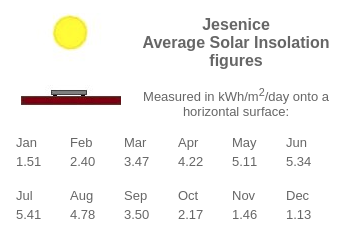
\includegraphics[width=.40\textwidth]{images/solar_energy.png}\hfill
    \caption{Produkovaná energie solárních panelů}
    \label{fig:solar_energy}
\end{figure}

Na obrázku~\ref{fig:solar_energy} je zachycena produkce energie solárních panelů na základě geografické polohy a jejich nasměrování vůči Slunci.\footnote{\url{http://solarelectricityhandbook.com/solar-irradiance.html?fbclid=IwAR0W-VqbCV1noK_vQZl4-U8a4ibCUvSwaAoGB0Nu52Dbzsnx_cmy2JlQMKU}} Na základě těchto dat, jsme spočítaly produkci energie všech panelů dle měsíců v roce.

\begin{center}
    \begin{table}[H]
        \centering
        \begin{tabular}{|c|c|}
            \hline
            Měsíc & Produkce energie jednoho panelu [$Kwh/$den] \\
            \hline
            \hline
            leden & 24.6 \\
            \hline
            únor & 39.1 \\
            \hline
            březen & 56.6 \\
            \hline
            duben & 68.8 \\
            \hline
            květen & 83.3 \\
            \hline
            červen & 87 \\
            \hline
            červenec & 88.2 \\
            \hline
            srpen & 77.9 \\
            \hline
            září & 57 \\
            \hline
            říjen & 35.4 \\
            \hline
            listopad & 23.8 \\
            \hline
            prosinec & 18.4 \\
            \hline
        \end{tabular}
        \caption{Produkce energie solárních panelů v závislosti na měsíci}
    \end{table}
\end{center}

Poruchovost solárních panelů je velmi nízka, v průměru 0.05\%. Jednou z hlavních příčin ovčem je silný vítr.\footnote{\url{https://news.energysage.com/average-solar-panel-failure-rate/}} My se ovšem nacházíme v lokalitě kde je vítr extrémně silný, budeme tedy uvažovat až 4x větší poruchovost, tedy \textbf{0.2\%}.\footnote{\url{http://www.meteocentrale.ch/en/europe/slovenia/weather-kredarica/details/S140080/}} Výměna solárního panelu by mohla trvat řádově měsíce, uvažujeme \textbf{3}.



\subsubsection{Akumulátory}

Skladování energie není úplně snadná záležitost. Uvažujeme, že \textbf{9/10} energie co uložíme budeme moci opět využít.\footnote{\url{https://www.energysage.com/solar/solar-energy-storage/what-are-the-best-batteries-for-solar-panels/}} Velikost akumulátorů v chatě odhadujeme celkem na \textbf{5000\,kWh}.\footnote{\url{https://www.wholesalesolar.com/solar-information/battery-bank-sizing}}



\subsection{Použité postupy pro vytvoření modelu a původ použitých metod/technologií}

Pro tvorbu simulačního modelu byl použit jazyk C++ s knihovnou SIMLIB.
\begin{itemize}
    \item C++\\
    \url{http://www.cplusplus.com/}
    \item SIMLIB\\
    \url{http://www.fit.vutbr.cz/~peringer/SIMLIB/}
\end{itemize}

Použité konstrukce a algoritmy jsou převážně inspirovány studijními materiály předmětu IMS.
\begin{itemize}
    \item IMS prezentace\\
    \url{https://www.fit.vutbr.cz/study/courses/IMS/public/prednasky/IMS.pdf}
    \item První democvičení\\
    \url{http://perchta.fit.vutbr.cz:8000/vyuka-ims/uploads/1/ims-demo1.pdf}
    \item Druhé democvičení\\
    \url{http://perchta.fit.vutbr.cz:8000/vyuka-ims/uploads/1/diskr2-2011.pdf}
    \item Dokumentace SIMLIB\\
    \url{http://www.fit.vutbr.cz/~peringer/SIMLIB/doc/SimLib-doc-2.ps}
    \item Doxygen dokumentace SIMLIB\\
    \url{https://www.fit.vutbr.cz/~peringer/SIMLIB/doc/html/}
    \item Příklady SIMLIB
    \url{http://www.fit.vutbr.cz/~peringer/SIMLIB/examples/}
\end{itemize}
